\documentclass[14pt, titlepage,fleqn]{extarticle}
\usepackage[T1,T2A]{fontenc}
\usepackage[utf8]{inputenc}

\usepackage{amsmath}
\usepackage[russian]{babel}

\usepackage{titlepage}
\usepackage[final]{pdfpages}
\usepackage{listings}
\usepackage{color}
\usepackage{graphicx}
\usepackage{float} 

\usepackage{caption}


\newcommand{\InsertGraf}[2]{
	\begin{figure}[H]
		\center{\includegraphics[width = 1\textwidth]{#1}}
		\caption{#2}
	\end{figure}
}

\definecolor{dkgreen}{rgb}{0,0.6,0}
\definecolor{gray}{rgb}{0.5,0.5,0.5}
\definecolor{mauve}{rgb}{0.58,0,0.82}


\lstset{frame=tb,
	language=Python,
	aboveskip=3mm,
	belowskip=3mm,
	showstringspaces=false,
	columns=flexible,
	basicstyle={\small\ttfamily},
	numbers=none,
	numberstyle=\tiny\color{gray},
	keywordstyle=\color{blue},
	commentstyle=\color{dkgreen},
	stringstyle=\color{mauve},
	breaklines=true,
	breakatwhitespace=true,
	tabsize=3
}

\begin{document}
	\selectlanguage{russian}
	

	\fefutitlepage{Б9119-02.03.01сцт}{Панченко Н.К.}{02}{июня}{22}
	
	
	\newpage
	
	\tableofcontents   
	\clearpage
	\section*{Введение}
	\addcontentsline{toc}{section}{Введение}
	Отчёт по лабораторной работе на тему <<Метод квадратного корня>>.	
	\newpage









	\section*{Метод квадратного корня}
	\addcontentsline{toc}{section}{Метод квадратного корня}
	Изучить и реализовать  метод квадратного корня для решения СЛАУ, а также описать работу алгоритма и
	привести результаты.

	\section*{Алгоритм}
	Метод используется для решения систем, у котроых матрица $A$ симметрична. В этом случает марицу $A$ можно разложить в произведение двух транспонированных друг другу треугольных матриц:
	\[A = S'S,\]
	\[S = \begin{bmatrix}
		s_{11} & s_{12} & \cdots & s_{1n} \\
		0 & s_{22} & \cdots & s_{2n} \\
		\cdots & \cdots & \cdots & \cdots \\
		0 & 0 & \cdots & s_{nn} \\
	\end{bmatrix}\]

	Формула для определения $s_{ij}:$
	\[s_{11} = \sqrt{a_{11}}, ~ s_{1j} = \dfrac{a_{1j}}{s_{11}},~ (j>1),\]
	\[s_{ii} = \sqrt{a_{ii} - \sum_{k = 1}^{i - 1}s^2_{ki}}~~(i>1),~~~ s_{ij} = \dfrac{a_{ij} - \sum_{k = 1}^{i - 1}s_{ki}s_{kj}}{s_{ii}} ~~ (j>1),\]
	\[s_{ij = 0} ~~~ (i>j).\]

	После того как матрица $S$ найдена, решают систему:
	\[S'y =b ,\]
	\newpage
	а затем находят неизвестные $x_1,x_2,\cdots,x_n$ из системы:
	\[Sx = y\]
	\[y_1 = \dfrac{b_1}{s_{11}}, ~~ y_i = \dfrac{b_i - \sum_{k = 1}^{i - 1}s_{ki}y_k}{s_{ii}}, (i > 1).\]
	\[x_n = \dfrac{y_n}{s_{nn}},~~ x_i = \dfrac{y_i - \sum_{k = i+1}^{n}s_{ik}x_k}{s_{ii}}, (i<n).\]
	
	\section*{Тесты}
	Возьмем матрицу из методички:
	\[A = \begin{pmatrix}
		1 & 3 & -2 & 0 & -2\\
        3 & 4 & -5 & 1 & -3\\
        -2 & -5 & 3 & -2 & 2\\
        0 & 1 & -2 & 5 & 3\\
        -2 & -3 & 2 & 3 & 4\\
	\end{pmatrix}\]
	Возьмем вектор:
	\[b =\begin{pmatrix}
		0.5\\
        5.4\\
        5.0\\
        7.5\\
    	3.3
	\end{pmatrix} \]
	Результаты:
	\begin{figure}[H]
		\center{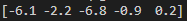
\includegraphics[width = 1\textwidth]{Screenshot_1.png}}
	\end{figure}

	\newpage
	Сравним с методом Гаусса:

	
	Результаты методом Гаусса:
	\begin{figure}[H]
		\center{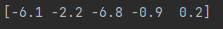
\includegraphics[width = 1\textwidth]{Screenshot_2.png}}
	\end{figure}
\end{document}